\documentclass{article}
\usepackage{graphicx} % Required for inserting images
\usepackage{amsmath}
\usepackage{amssymb}
\usepackage{amsthm}
\usepackage{mathrsfs}
\usepackage{hyperref}
\usepackage{tikz}
\usetikzlibrary{automata, arrows.meta, positioning}

\usepackage{diagbox}


% PUT COMMANDS HERE
% ------------------------------
\newcommand{\question}[1]{\item (\textbf{#1})}
\newcommand{\dif}{\mathop{}\!\mathrm{d}}

\theoremstyle{remark}
\newtheorem*{remark}{Remark}
% ------------------------------
\title{Math 239 Fall 2023 Tutorial: Cache of Combinatorial Curiosities}
\author{Alex Kroitor}

\begin{document}



% \date{2023 Sep. 21/22}
\maketitle

\begin{abstract}
    This is a list of 239-adjacent questions that I find fun/interesting. Try these at your own risk! Note these are not useful for $239$ beyond making you feel more intimately connected with the material.
\end{abstract}

\begin{enumerate}
    \question{Formal Derivatives}

    Consider a generating function
    \begin{align*}
        A(x) = \sum_{i=0}^\infty a_i x^i = a_0 + a_1 x + a_2 x^2 + a_3 x^3 + \cdots.
    \end{align*}
    We define the \textit{formal derivative} of $A(x)$ to be
    \begin{align*}
        \frac{\dif}{ \dif x} A(x) = \sum_{i = 1}^\infty i a_i x^{i-1} = 1 a_1 + 2 a_2 x + 3 a_3 x^2 + 4 a_4 x^3 + \cdots.
    \end{align*}
    \begin{enumerate}
        \item Find $[x^n] \left[ \frac{\dif}{\dif x} A(x) \right]$.
        \item Find $[x^n] \left[ x \frac{\dif }{\dif x} A(x)  \right]$.
        \item Using the \textit{formal derivative} as a ``normal derivative", ie treating the derivative like you would in a first calculus course, find the generating function for the following sequences.
        \begin{enumerate}
            \item $a_n = n$.
            \item $a_n = n^2$.
            \item $a_n = n^k$ for any fixed $k \geq 1$.
        \end{enumerate}
    \end{enumerate}
    \begin{remark}
        The last one might be hard/impossible, but it turns out if you care only about the \textit{asymptotic behaviour} of $a_n$, that is you want $a_n$ to be approximately $n^k$ for large enough $n$, it is much easier. A result from \textit{analytic combinatorics} says that one example of a generating function for a sequence like this is $\frac{k!}{(1-x)^{k+1}}$ (in fact by the math software Sagemath, then $[x^{1000}] \frac{4!}{(1-x)^5} \approx 1.01004513028955 \cdot (1000)^4$, which shows that at $n=1000$ there is only about a $1 \%$ error).
    \end{remark}

    \question{A Second GF for Binomial Coefficients}
    
    Single-variate generating functions are familiar to us at this point in the course. We can similarly define bi-variate generating functions as formal power series
    \begin{align*}
        A(x,y) =  \sum_{i \geq 0} \sum_{j \geq 0} a_{i,j} x^i y^j.
    \end{align*}

    A familiar GF to us is the GF for binomial coefficients with respect to ``$k$"
    \begin{align*}
        \sum_{k \geq 0} \binom{n}{k} x^k = (1+x)^n.
    \end{align*}
    Using this, and the notion of a bi-variate generating function, find a closed form for the GF for binomial coefficients with respect to ``$n$"
    \begin{align*}
        \sum_{n \geq 0} \binom{n}{k} y^n.
    \end{align*}

    \question{Counting Binary Trees and Dyck Paths}

    Define a full binary tree to be a binary tree where each vertex has either $0$ or $2$ children. Often we can realize trees and other combinatorial structures recursively. Probably the most popular example is realizing that a full binary tree is either empty, or a vertex followed by two full binary trees.

    \begin{enumerate}
        \item Justify that this gives us the GF relationship
        \begin{align*}
            B(x) = 1 + x \cdot B(x) \cdot B(x) = 1 + xB(x)^2.
        \end{align*}
        Solve this for $B(x)$ and justify which of the two solutions is the legitimate one.
        \item Using the generalization of binomial expansion in \url{https://en.wikipedia.org/wiki/Binomial_series}, find a closed-form expression for the number of binary trees with $n$ vertices (ie find $[x^n]B(x) =: C_n$).
    \end{enumerate}
    After a lot of algebra this is very amazingly the Catalan numbers! These numbers pop up in the wild quite a lot.
    \begin{enumerate}
        \item[(c)] A \textbf{Dyck path} of length $2n$ is a path from $(0,0)$ to $(n,n)$ using the steps $(1,0)$ and $(0,1)$ that always stays below (it is allowed to touch) the diagonal $x=y$. For examples see \url{https://math.mit.edu/~apost/courses/18.204-2016/18.204_Gabriella_Baracchini_final_paper.pdf}. Think about what these look like, then show that the generating function for Dyck paths satisfies a similar relation as the one in $(a)$. Conclude that the Catalan number $C_n$ is equal to the number of Dyck paths of length $2n$.
        \item[(d)] We have proven by comparing generating functions that the number of full binary trees with $n$ nodes is equal to the number of Dyck paths of length $2n$ (which is turn is the $n$-th Catalan number). This is an ``unenlightening" proof, in the sense that the relationship between the two is unclear. We would prefer a more explicit bijection between the two. Come up with a bijection between full binary trees with $n$ nodes and Dyck paths with length $2n$.
    \end{enumerate}
    
    \question{Automata and Languages}
    There is a very strong relationship between regular expressions and computer scientific models. This is expressed through the relationship between regular expressions and so-called \textbf{finite-state automata}. Morally these are models of machines that have finitely many possible states, and depending on the input you feed to the machine, transitions from one state to another. More formally a finite-state automaton is (pulled from Wikipedia) a quintuple $(\Sigma , S , s_0 , \delta, F)$, where
    \begin{itemize}
        \item $\Sigma$ is the input alphabet (a finite non-empty set of symbols);
        \item $S$ is a finite non-empty set of states;
        \item $s_{0}$ is an initial state, an element of S;
        \item $\delta$ is the state-transition function: $\delta : S \times \Sigma \to S$;
        \item $F$ is the set of final states, a (possibly empty) subset of $S$.
    \end{itemize}
    Usually we default to $\Sigma = \{ 0,1 \}$. We can write these in a nice way by drawing them visually. For example
    \begin{center}
        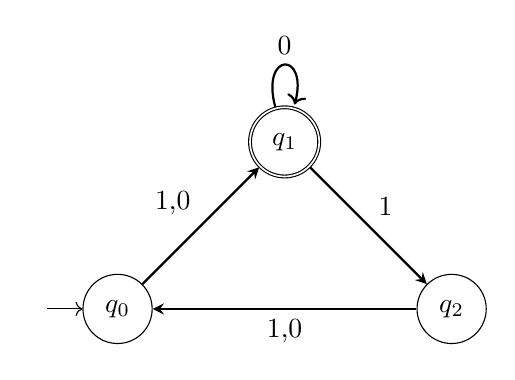
\begin{tikzpicture} [node distance = 3cm, on grid, auto]

\node (q0) [state, initial, initial text = {}] {$q_0$};
\node (q1) [state, accepting, above right = of q0] {$q_1$};
\node (q2) [state, below right = of q1] {$q_2$};

\path [-stealth, thick]
	(q0) edge node {1,0}   (q1)
	(q1) edge node {1}   (q2)
	(q1) edge [loop above]  node {0}()
	(q2) edge node {1,0} (q0);
\end{tikzpicture}
    \end{center}
    is a visual representation of the FSA with $\Sigma = \{ 0,1\}$, $S = \{ q_0 , q_1, q_2\}$, $s_0 = q_0$ (indicated by the little arrow pointing to it), $\delta$ represented by the arrows with numbers above them, and $F = \{ q_1 \}$ (indicated by the double circle).
    Given an FSA we say that the set of strings that ends at $F$ is the language accepted by it. It turns out that for every regular language there is an FSA that accepts exactly that language, and that the language accepted by FSAs are always regular (and so there's a one-to-one correspondence between regular languages and FSAs).
    \begin{enumerate}
        \item Give the regular expression that is accepted by the FSA above.
        \item Argue that the language $\{\, 0^n 1^n : n \in \mathbb{N} \, \}$ cannot be expressed with a regular language by convincing yourself that it cannot be written with an FSA (note: there is a way to prove this, but it requires some more machinery).
    \end{enumerate}
    It turns out that other languages correspond to different kinds of automata. An example of this is context-free languages (more or less a language that uses a recursive definition) and what are called push-down automata. This is an FSA with the added condition that you can ``push" and ``pop" elements from a stack. These are more general than the FSA constructions.
    \begin{enumerate}
        \item[(c)] Read the Wikipedia article on push-down automata, and then write a PDA that accepts $\{\, 0^n 1^n : n \in \mathbb{N} \, \}$. This shows that this language is in fact a context-free language but not a regular languag (note that the answer to this question is on the Wikipedia page for PDAs, but you should convince yourself that it makes sense).
    \end{enumerate}
    \question{Fibonacci Recurrences}
    Consider the Fibonacci recurrence given by $f_{n+2} = f_{n+1} + f_n$, where $f_0 = 0$ and $f_1 = 1$. As we know from class and partial fraction decomposition, this has the closed form
    \begin{align*}
        f_n = \frac{(1+\sqrt{5})^n}{2^n \sqrt{5}} -  \frac{(1-\sqrt{5})^n}{2^n \sqrt{5}}.
    \end{align*}
    Notice that the second term goes to $0$ as $n \to \infty$.
    \begin{enumerate}
        \item Find a general formula for the Fibonacci-like recurrence given by $f_{n+2} = f_{n+1} + f_n$, where $f_0 = a$ and $f_1 = b$, where $a,b \in \mathbb{R}$. Then the set of initial conditions is $\mathbb{R}^2$. Conclude that there is a one-dimensional subspace of $\mathbb{R}^2$ such that $f_n \to 0$ when the initial conditions are in this subspace (ie there is a line of possible initial values that make $f_n$ tend to $0$). Compute the line orthogonal to this one. What happens to our sequence when our initial conditions are in this orthogonal line?
        \item (hard) Find a closed form for the Tribonacci numbers, defined by $f_{n+3} = f_{n+2} + f_{n+1} + f_n$, where $f_0 = a_0 , f_1 = a_1 , f_2 = a_2$. Then the set of initial conditions is $\mathbb{R}^3$. This has a (possibly trivial) subspace of initial conditions that make $f_n \to 0$. What is the dimension of it?
        \item Can you find the dimension of the subspace of initial conditions that make $f_n \to 0$ for arbitrary $k$-Fibonacci numbers?
    \end{enumerate}
    This last one seems hard. From my own experimentation, it seems that there is always exactly one root of $1-x-x^2 - \cdots - x^k$ with norm less than one, and that every root is simple. Thus we only need to care about this single root (note this root tends to $0.5$, which indicates our numbers will tend to having exponential growth $2^n$). Then from how partial fractions works, this will give a monomial with a linear combination of the $k$ initial conditions as a coefficient on top (in fact this follows from $239$ material). Then it is impossible to have no initial conditions in our linear combination. Thus if we consider our linear combination as a $1 \times k$ matrix, since this a non-zero matrix it follows from the rank-nullity theorem that the nullity is $k-1$. It thus follows that the vector space of initial conditions that lead to $f_n \to 0$ is a $k-1$ dimensional linear subspace of $R^{k}$.

    \question{Moore Graphs}
    We often try to import the language for geometric shapes over to graphs. In this light we define the \textbf{distance} between two vertices as
    \begin{align*}
        \operatorname{dist} (u,v) = \min_{\gamma \in path(u,v)} \operatorname{length}(\gamma)
    \end{align*}
    where $path(u,v)$ is the set of all paths from $u$ to $v$, and the length of a path is the number of edges you cross in the path. We define the \textbf{diameter} of a graph to be
    \begin{align*}
        diam(G) = \max_{u,v \in G} \operatorname{dist} (u,v).
    \end{align*}
    This is a measure of how ``spread out" our graph is; if our graph has lots of edges you expect the diameter to be high, and if the graph has few edges you expect a low diameter.
    
    Let $G$ be $d$-regular and have diameter $k$. Show that
    \begin{align*}
        |V(G)| \leq 1 + d \sum_{i=1}^{k} (d-1)^{i-1}.
    \end{align*}
    A graph in which we achieve equality is known as a \textbf{Moore graph}. Some examples of Moore graphs are odd cycles, complete graphs, and the Petersen graph.
\question{Hadwiger-Nelson}
    Until now we have been dealing with finite graphs, but we do not run into any problem extending to infinite graphs. In particular one might want to think about the chromatic number, i.e. the minimum number of colours one needs to use to colour a graph so that no two adjacent vertices share a colour.
    \begin{enumerate}
        \item Consider the graph $G_1$ on $\mathbb{Z}$ with two vertices being adjacent iff their corresponding numbers are off by one. For example $3$ is adjacent to only $2$ and $4$. Find the chromatic number of $G_1$.
        % \item Consider the graph $G_2$ on $\mathbb{Z}^2$ with two vertices being adjacent iff they differ in exactly one coordinate by exactly one. For example $(2,3)$ is adjacent to only $(1,3), (3,3), (2,2), (2,4)$. Find the chromatic number of $G_2$.
        \item Consider the graph $G_n$ on $\mathbb{Z}^n$ where two vertices are adjacent iff they differ in exactly one coordinate by exactly one. Find the chromatic number of $G_n$.
        \item Consider the graph $R_1$ with base set $\mathbb{R}$, with two vertices being adjacent if they have distance one. Find the chromatic number of this graph.
    \end{enumerate}
    Now that we have some practice let's prove some interesting results. Let $G$ be the graph on $\mathbb{R}^2$ where two points are adjacent if their (Euclidean) distance is $1$.
    \begin{enumerate}
        \item[(d)] Show that the chromatic number of $G$ is at most $7$ by finding a colouring of $G$ that uses $7$ colours.
        \item[(e)] Show that the chromatic number of $G$ is at least $4$ by finding a subset of $G$ that cannot be coloured with less than $4$ colours.
    \end{enumerate}
    This shows that the chromatic number of $G$ is either $4,5,6,7$. A bit shockingly, the biologist de Grey in 2018 showed that it cannot be $4$. Finding the exact chromatic number of $G$ is known as the Hadwiger-Nelson problem.

    \question{Complete $k$-partite Graphs} We say a graph $G=(V,E)$ is \textbf{$k$-partite} if we can partition $V = V_1 \sqcup \cdots \sqcup V_k$ ($\sqcup$ indicates \textit{disjoint} union, and the $V_j$ are called \textit{parts}) such that there are no edges between distinct elements of $V_j$ (where $j = 1, \cdots, k$). Find a tight bound on the number of edges in a $k$-partite graph with $kn$ vertices, and say when this tight bound occurs.

    \begin{remark}
        This should in particular agree with the $k=2$ case and the $k=3$ case ($n^2$ and $3 n^2$).
    \end{remark}

    \question{Exotic Cubes} Let $C_{n,m}$ be the graph where the vertices are the elements of $\{ 0, 1 , \cdots, m-1\}^n$, and where there is an edge between $v_1$ and $v_2$ iff $v_1 $ and $v_2$ differ by exactly $1$ in exactly one coordinate. Note this is the graph $(P_m)^{\square n}$. What is the number of edges in this graph?
    \begin{remark}
        I will write down my solution here for those curious. The argument here is simple degree counting. There are $m^n$ points in this graph. Let the codimension of a vertex be the codimension of a vertex be the number of vectors $e_j$ such that either adding or subtracting $e_j$ yields a point off your graph. For example if $n=3$ the codimension of a point at a corner is $3$, a point on an edge but not a corner is $2$, a point on a face but not an edge or a corner is $1$, and a point in the interior is $0$. The degree of a point with codimension $i$ is $2n-i$. Now we must count the number of points of a given codimension. First note that if we want a codim $i$ subspace we simply pick $i$ of the $n$ basis vectors we have to exclude, which gives us $\binom{n}{i}$. Then note that if we exclude a vector, then we get another copy of our subspace by adding our excluded $e_i$. There are $2^i$ such shifts by excluded vectors. It follows that there are $2^i \binom{n}{i}$ subspaces of codim $i$ appearing in our graph. Finally the number of points in each face is $(m-2)^{n-i}$, since we are only allowed coordinates in the range $\{ 1 , \cdots, m-2 \}$ (otherwise we are on a different codimension face), and since we are allowed to move in $n-i$ dimensions. It follows that there are exactly $(m-2)^{n-i} 2^i \binom{n}{i}$ points of codimension $i$. Note that summing verifies that we have $m^n$ points in total. It follows that
        \begin{align*}
            |E| = \frac{1}{2} \sum_{j=0}^n (2n - j) (m-2)^{n-j} 2^j \binom{n}{j}.
        \end{align*}
        Another grad student (Nick) pointed out that this can be counted another (admittedly much easier) way to get
        \begin{align*}
            |E| = m^{n-1} (m-1) n.
        \end{align*}
        I suppose this implies a combinatorial identity
        \begin{align*}
            m^{n-1} (m-1) n = \frac{1}{2} \sum_{j=0}^n (2n - j) (m-2)^{n-j} 2^j \binom{n}{j}.
        \end{align*}
    \end{remark}
    \question{The Pentagon Problem}
    Let $G$ be a $5$-cycle (a pentagon) with vertices enumerated $1 ,2,3,4,5$ in a circle. Let $c = (c_1 , c_2, c_3, c_4, c_5)$ denote certain numbers we put on vertex $1,2,3,4,5$ respectively (so vertex $3$ has the value $c_3$ on it). We let $c_j \in \mathbb{Z}$, but we require that $c_1 + c_2 + c_3 + c_4 + c_5 \geq 1$. Now play the following game:
    \begin{itemize}
        \item[] If we have all $c_j>0$ then we have won. Otherwise pick a vertex $j$ with $c_j < 0$. Then ``activate" the vertex to get a new configuration $c'$ with
        \begin{align*}
            c'_i = \begin{cases}
                c_i & \text{if $i$ is not adjacent to $j$},\\
                c_{i} + c_j & \text{if $i$ is adjacent to $j$},\\
                c_{i} - 2c_i & \text{if $i = j$}.
            \end{cases}
        \end{align*}
        Then continue the game from the start with the configuration $c'$.
    \end{itemize}
    Show that we always win, so we always reach a state where $c_j > 0$ for all initial $c$'s.

    This problem is sourced from \textit{The Mathematics of Chip-Firing} by Klivans (problem $2.8.17$). I have no idea how to do it.
    \question{Spectral Graph Theory}
    The Laplacian operator on $\mathbb{R}^n$, which acts on functions $\mathbb{R}^n \to \mathbb{R}$ by sending $f$ to $\Delta f = \sum_{i = 1}^n \frac{\partial^2 f}{\partial x_i^2}$. The Laplacian operator notionally measures how much $f$ at $p$ differs from points near $p$. It turns out this plays a large role in a theory of mathematics called spectral theory, which is concerned with finding functions $f$ such that $\Delta f = \lambda f$ (so-called ``eigenfunctions").

    There is a graph theory equivalent of the Laplacian. Let $G$ be a graph with $n$ vertices, labelled $1 , \cdots , n$. Then Define the \textbf{degree matrix} $D_G$ of $G$ as the $n \times n$ matrix
    \begin{align*}
        D_G(i,j) = \begin{cases}
            \deg (v_i) & \text{ if } i=j,\\
            0 & \text{ else}.
        \end{cases}
    \end{align*}
    Define as well the \textbf{adjacency matrix} $A_G$ of $G$ as the (symmetric) $n \times n$ matrix
    \begin{align*}
        A_G(i,j) = \begin{cases}
            -1 & \text{ if } v_i v_j \in E,\\
            0 & \text{ else}.
        \end{cases}
    \end{align*}
    Now finally define the \textbf{graph Laplacian} of $G$ as $L = L_G = D_G - A_G$. Since this is an $n \times n$ real symmetric matrix, there are $n$ real eigenvalues (counted with multiplicity). This is exactly the provenance of \textbf{spectral graph theory}. We call the multiset of eigenvalues the \textbf{spectrum} of a graph, and often write them in increasing order $\lambda_1 \leq \cdots \leq \lambda_n$ (so that $\lambda_1$ is the lowest eigenvalue of $G$).
    \begin{enumerate}
        \item Argue that for any $G$ then $L (1, \cdots, 1)^T = 0$, and so $0$ is always an eigenvalue of $G$.
        \item Find the spectrum of $K_n$, $K_{n,n}$, $P_n$, $C_n$, the star graph $S_n$, and the $n$-cube $Q_n$.
        \item Prove that if $G$ is connected then $\lambda_1> 0$.  Further show that if $\lambda_i = 0$ and $\lambda_{i+1} \neq 0$ then $G$ has exactly $i+1$ connected components.
    \end{enumerate}
\end{enumerate}




\end{document}
